\documentclass[12pt,a4]{article}
\usepackage[left=1.8cm,right=1.8cm,top=32mm,columnsep=20pt]{geometry}

\usepackage[utf8]{inputenc} %Formato de codificación
\usepackage[spanish, es-tabla, es-nodecimaldot]{babel}
\usepackage{amsmath} %paquete para escribir ecuaciones matemáticas
\usepackage{float} %Para posicionar figuras
\usepackage{graphicx} %Para poder poner figuras
\usepackage{tikz}
\usetikzlibrary{positioning}
\usetikzlibrary{shapes.geometric, decorations.pathreplacing}

\title{Encontrando el coeficiente de fricción dinámica}
\author{Francisco Carruthers, Facundo Firpo y Joel Jablonski\\ [2mm]
\small \texttt{\{fcarruthers, ffirpo, jjablonski\}@udesa.edu.ar}\\
\small Fisica I, tutorial Vinograd}
\date{2do Semestre 2024}


\begin{document}

\maketitle

\begin{abstract}
    Se investigó el coeficiente de fricción dinámica entre un trineo y varias superficies utilizando un sistema de trineo, soga y polea. En primer lugar, se realizó una calibración previa del sistema, ajustando los sensores y asegurando que las lecturas de posición y tiempo fueran precisas. A continuación, se varió la masa del trineo y se midió la aceleración para calcular el coeficiente de fricción dinámica ($\mu_d$) en diferentes superficies. Las superficies evaluadas incluyeron el trineo sobre madera, trineo sobre papel y papel sobre papel. Los valores obtenidos para el $\mu_d$ fueron: 0.4 ± 0.1 para madera y trineo, 0.45 ± 0.03 para papel y trineo, y 0.5 ± 0.2 para papel y papel. [Los resultados demostraron que la superficie tiene un impacto significativo en la fricción dinámica del sistema.] CORREGIR
\end{abstract}

\section{Introducción}

La fricción es una fuerza de resistencia que actúa en oposición al movimiento relativo entre dos superficies en contacto. Existen dos tipos principales de fricción: la fricción estática, que previene el movimiento, y la fricción dinámica (o cinética), que actúa cuando el objeto ya está en movimiento. En este experimento, nos centraremos en la fricción dinámica, cuyo coeficiente, denotado como \(\mu_d\), se define como la relación entre la fuerza de fricción y la fuerza normal ejercida sobre el objeto:

\[
\vec{F_r} = \mu_d \cdot \vec{F_n}
\]

donde \(\vec{F_r}\) es la fuerza de fricción y \(\vec{F_n}\) es la fuerza normal, que para superficies horizontales es equivalente al peso del objeto en contacto con la superficie. Este coeficiente depende del tipo de materiales en contacto y su textura.

La determinación del $\mu_d$ es fundamental en la física aplicada, ya que afecta el diseño de sistemas mecánicos, el análisis de movimientos y la estabilidad de objetos en distintas superficies. En este contexto, comprender la relación entre la fuerza de fricción y la aceleración del objeto es crucial. Para este experimento, utilizamos la segunda ley de Newton, que establece que la fuerza neta que actúa sobre un objeto es proporcional a la masa del objeto y su aceleración:

\[
\vec{F} = m \cdot \vec{a}
\]

\section{Practica experimental}

\begin{figure}[H]
    \centering
    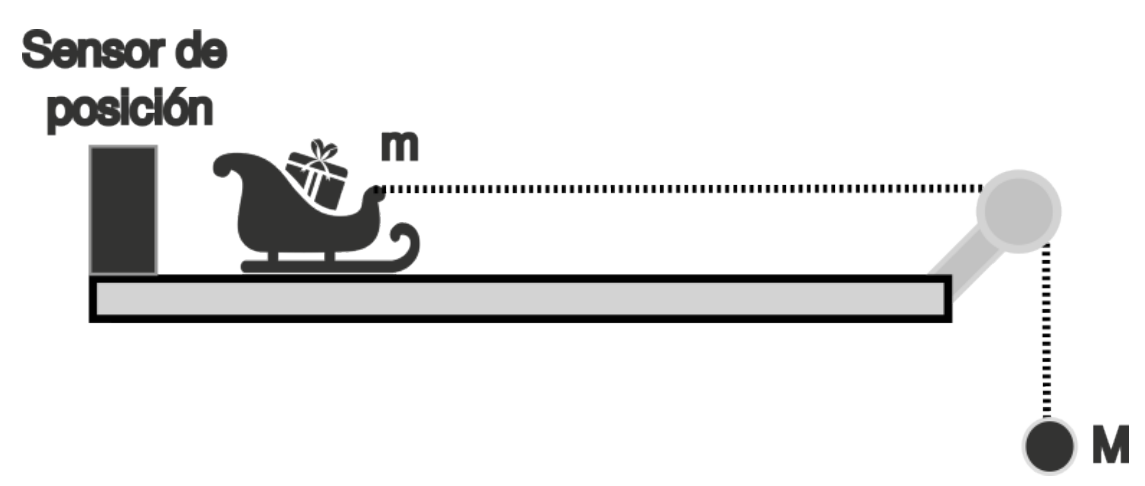
\includegraphics[width=0.9\linewidth]{esquema.png}
    \caption{Esquema experimental para la propuesta. La masa m y M son variables.}
    \label{fig:system}
\end{figure}

Dispusimos de un sistema de trineo, soga, polea y sensor de posicion. El sistema se muestra en la Figura \ref{fig:system}. La masa del trineo y la masa total del sistema son variables, lo que nos permite explorar varias configuraciones para ver como las masas afectan al $\mu_d$.

En primera instancia, nos propusimos calibrar el sensor. El sensor envia una señal, la cual rebota contra el trineo y vuelve al sensor. La señal es proporcional a la distancia entre el sensor y el trineo. La calibración consistió en determinar la pendiente y la ordenada al origen de la relación entre la señal y la distancia. Estos valores son necesarios para determinar la distancia recorrida por el trineo en función de la señal del sensor. Para ello, con una regla fuimos ubicando el trineo a distancias conocidas y anotamos la señal del sensor. Luego, ajustamos una recta a los datos obtenidos.

Una vez calibrado el sensor, procedimos a realizar el experimento. Primero, colocamos el trineo sobre la mesa de madera y lo dejamos deslizar. Medimos la distancia recorrida por el trineo en función del tiempo. Este procedimiento lo repetimos para $m = 161 \pm 1 g$ y $M = 72 \pm 1 g$, $m = 243 \pm 1 g$ y $M = 95 \pm 1 g$ y $m = 109 \pm 1 g$ y $M = 46 \pm 1 g$. Con estos datos, haciendo un ajuste cuadratico, podemos determinar la aceleración del trineo. 
Luego, repetimos el experimento pero pegandole un papel a la mesa. Usamos $m = 161 \pm 1 g$ y $M = 72 \pm 1 g$, $m = 243 \pm 1 g$ y $M = 95 \pm 1 g$ y $m = 109 \pm 1 g$ y $M = 46 \pm 1 g$. 
Por ultimo, pegamos un papel al trineo y repetimos el experimento.

Combinando esta ecuación con la expresión de la fuerza de fricción podemos deducir que la aceleración del trineo estará influenciada por el coeficiente de fricción y la masa total del sistema. Podemos despejar la formula como:

\begin{equation}
    \mu_d = \frac{\vec{a} \cdot (M + m) + M \cdot \vec{g} }{m \cdot \vec{g}}
    \label{eq:mu_d}
\end{equation}

En nuestro caso, el sistema se conforma de un trineo y varias superficies, lo que nos permite explorar cómo el coeficiente de fricción cambia según el material.

Armamos el sistema de la siguiente manera:

Dispusimos de los siguientes materiales para realizar el experimento:

% \begin{table}[H]
%     \centering
%     \begin{tabular}{|c|c|}
%         \hline
%         \textbf{Objeto} & \textbf{Masa(g)} \\
%         \hline
%         Pesa dorada & $72 \pm 1$ \\
%         Pesa plateada & $23 \pm 1$ \\
%         Pesa madera & $6 \pm 1$ \\
%         Trineo & $109 \pm 1$ \\
%         Metro & $134 \pm 1$ \\
%         \hline
%     \end{tabular}
%     \label{tab:mediciones}
% \end{table}

\section{Calibración}

Para calibrar el sistema, empleamos un sistema de referencia basado en mediciones de distancia que oscilan entre 15 cm y 35 cm, utilizando una regla previamente calibrada como
 instrumento de medición. El sensor en cuestión proporciona unidades arbitrarias. Al comparar estos valores con las distancias reales, determinamos que existe una relación lineal
  entre la señal del sensor y la distancia medida. Con esta información, realizamos un ajuste lineal a los datos obtenidos, lo que nos permitió derivar una ecuación de la recta que
   describe esta relación. Los valores resultantes de este ajuste, junto con sus respectivas incertidumbres, se presentan a continuación:

\begin{figure}[H]
    \centering
    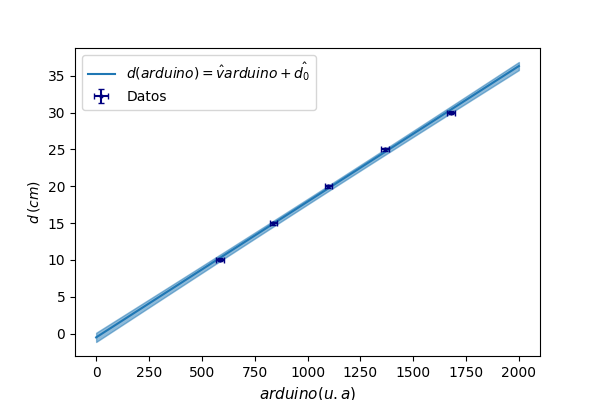
\includegraphics[width=0.8\linewidth]{Calibracion.png}
    \caption{Calibracion del sistema mediante la comparacion de la señal del sensor con la distancia real}
    \label{fig:calibracion}
\end{figure}

El grafico de la Figura \ref{fig:calibracion} muestra la recta:

\begin{equation}
    dist(a) = (0.0184 \pm 0.0005) \cdot a + (-0.5 \pm 0.5) cm
    \label{eq:dist}
\end{equation}

La pendiente representa la tasa de cambio de la señal del sensor con respecto a la distancia medida, indicando que por cada centímetro de distancia, la señal del sensor cambia en
 aproximadamente 0.0184 unidades arbitrarias. La incertidumbre asociada a la pendiente, de ±0.0005 unidades arbitrarias, refleja la precisión del ajuste lineal realizado.


Por otro lado, la ordenada al origen de -0.5 cm, con una incertidumbre de ±0.5 cm, sugiere que cuando la señal del sensor es cero, la distancia medida sería aproximadamente -0.5 cm.
 Esta ordenada al origen negativa puede interpretarse como un desplazamiento sistemático en las mediciones del sensor, posiblemente debido a factores como el posicionamiento inicial 
 del sensor o pequeñas desviaciones en la calibración de la regla utilizada.

\section{Resultados}

\subsection{Posicion}

Registramos la distancia recorrida y el tiempo empleado para calcular la velocidad y la aceleración del trineo. Al tener estas mediciones, podemos evaluar cómo factores como la
 fricción influyen en el rendimiento del trineo en las diferentes superficies.

Posteriormente, realizamos un ajuste cuadrático a los datos obtenidos. Este ajuste nos permitió analizar si una relación no lineal describe mejor el comportamiento del trineo.
 Al incluir un término cuadrático en el modelo, pudimos capturar posibles curvaturas en los datos que un ajuste lineal no podría representar adecuadamente. Este enfoque nos
  proporcionó una visión más precisa del movimiento del trineo.

\subsubsection*{Madera y Trineo}

En un primer caso, dejamos que el trineo se deslizara sobre la superficie de una mesa de madera. Este experimento inicial nos permitió observar cómo la fricción de la madera
 afecta el movimiento del trineo.\\

\begin{figure}[H]
    \centering
    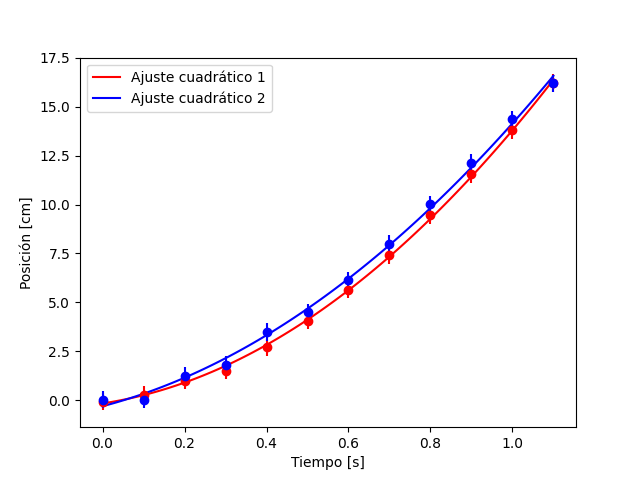
\includegraphics[width=0.44\linewidth]{ajuste2_PisoMaderaMPB_O.png}
    \caption{$m = (243 \pm 1) g, M = (95 \pm 1) g$}
    \label{fig:M_OP piso trineo}
\end{figure}

Del ajuste cuadratico visto en la figura \ref{fig:M_OP piso trineo} obtenemos una ecuacion de la forma:

\[
pos(t) = (0.11 \pm 0.01) \frac{cm}{s^2} \cdot t^2 + (0.03 \pm 0.01) \frac{cm}{s} \cdot t + (-0.002 \pm 0.002) cm
\]

\subsubsection*{Papel y trineo}

Luego, cubrimos la superficie de la mesa con papel y repetimos el experimento. Esto nos permitió comparar cómo la fricción del papel afecta el movimiento del trineo en comparación con la madera.

\begin{figure}[H]
    \centering
    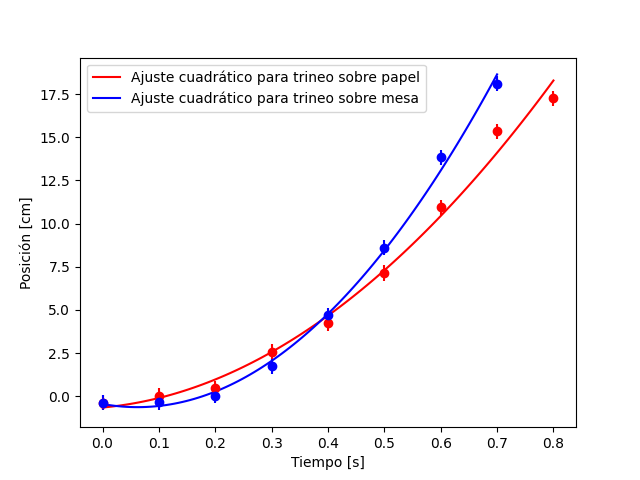
\includegraphics[width=0.44\linewidth]{ajuste2_PisoHojaM_OP.png}
    \caption{$m = (243 \pm 1) g, M = (95 \pm 1) g$}
    \label{fig:M_OP piso hoja}
\end{figure}


Del ajuste cuadratico visto en la figura \ref{fig:M_OP piso hoja} obtenemos una ecuacion de la forma:

\[
pos(t) = (0.19 \pm 0.02) \frac{cm}{s^2} \cdot t^2 + (0.08 \pm 0.02)\frac{cm}{s} \cdot t + (-0.004 \pm 0.004) cm
\]

\subsubsection*{Papel y Papel}

Por último, adherimos un papel adicional al trineo y repetimos el experimento. Esta variación nos permitió observar cómo la fricción entre dos superficies de papel afecta el movimiento del trineo, en comparación con las pruebas anteriores.

\begin{figure}[H]
    \centering
    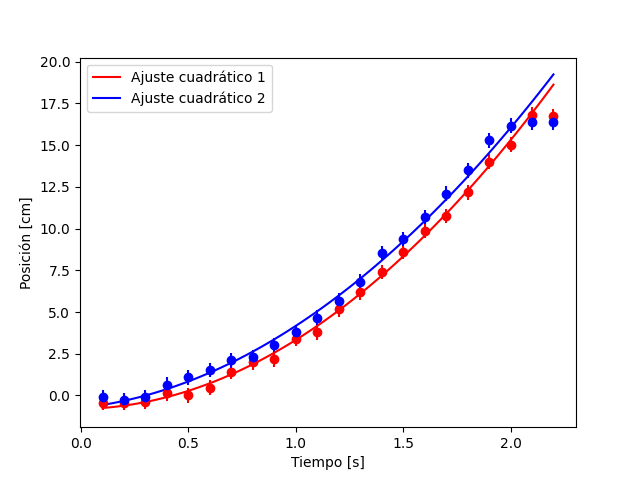
\includegraphics[width=0.44\linewidth]{ajuste2_PapelPapelM_O.png}
    \caption{$m = (243 \pm 1) g, M = (72 \pm 1) g$}
    \label{fig:M_O papel papel}
\end{figure}

Del ajuste cuadratico visto en la figura \ref{fig:M_O papel papel} obtenemos una ecuacion de la forma:

\[
pos(t) = (0.040 \pm 0.004) \frac{cm}{s^2} \cdot t^2 + (0.001 \pm 0.009) \frac{cm}{s} \cdot t + (-0.008 \pm 0.004) cm
\]

\subsection{Obtencion del $\mu_d$}

Sacando un promedio de los valores obtenidos de \ref{eq:mu_d} usando cada aceleración obtenemos un valor de $\mu_d$ para cada superficie.

\begin{figure}[H]
    \begin{minipage}{0.5\textwidth}
        \centering
        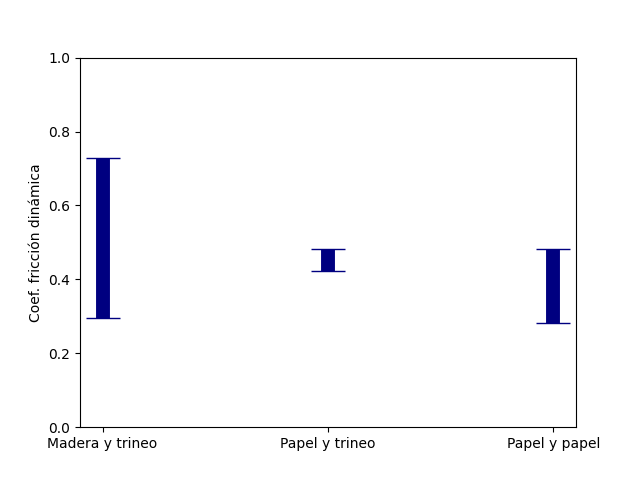
\includegraphics[width=0.9\linewidth]{ud_Combined.png}
        \caption{Promedio de $\mu_d$ para cada superficie}
        \label{fig:mu_d promedio}
    \end{minipage}\hfill
    \begin{minipage}{0.5\textwidth}
        \centering
        \begin{table}[H]
            \centering
            \begin{tabular}{|c|c|}
                \hline
                \textbf{Superficie} & \textbf{$\mu_d$}\\
                \hline
                Madera y trineo & $0.4 \pm 0.1$\\
                Papel y trineo & $0.45 \pm 0.03$ \\
                Papel y Papel & $0.5 \pm 0.2$ \\
                \hline
            \end{tabular}
            \caption{Valores de $\mu_d$ y sus incertezas para cada superficie}
            \label{tab:mu_d}
        \end{table}
    \end{minipage}
\end{figure}

\section{Conclusiones}

A través de las mediciones de aceleración en diversas configuraciones de masa y superficie, se obtuvieron valores para el $\mu_d$, destacándose variaciones entre las diferentes superficies analizadas.

Los resultados obtenidos evidencian que la fricción varía dependiendo de la textura de las superficies en contacto. Por ejemplo, el valor de $\mu_d$ en la superficie de madera fue de 0.4 ± 0.1, mientras que en papel sobre papel fue mayor, alcanzando un promedio de 0.5 ± 0.2. Esta variación en el coeficiente es indicativa de la influencia de la rugosidad y la naturaleza del material en la interacción de fricción.

Por las incertezas de los resultados, podemos comprender la importancia de las condiciones experimentales y cómo pequeñas variaciones pueden impactar en los resultados, reforzando el valor de una correcta medición y calibración en estudios físicos.


\end{document}